\documentclass[11pt,letterpaper]{article}
\usepackage[T1]{fontenc}
\usepackage[utf8]{inputenc}
\usepackage{lmodern}
\usepackage[margin=0.75in,headheight=15pt,headsep=18pt,footskip=24pt]{geometry}
\usepackage{microtype,amsmath,amssymb,mathtools,graphicx,booktabs,tabularx,array}
\usepackage{xcolor,tikz,tcolorbox,enumitem,fancyhdr,titlesec,listings,caption,hyperref}
\newcolumntype{Y}{>{\raggedright\arraybackslash}X}
\usetikzlibrary{arrows.meta,positioning,calc,fit}
\definecolor{navy}{HTML}{17324D}
\definecolor{teal}{HTML}{087E8B}
\definecolor{pale}{HTML}{EDF6F7}
\definecolor{orange}{HTML}{D87828}
\definecolor{graytext}{HTML}{526171}
\definecolor{lightgray}{HTML}{F3F5F7}
\hypersetup{colorlinks=true,linkcolor=teal,urlcolor=teal,citecolor=teal,pdftitle={EC523 Project A: Think Again, Segment Better},pdfauthor={EC523 course staff},pdfsubject={Looped transformer road segmentation project; instructor review draft}}
\pagestyle{fancy}
\fancyhf{}
\fancyhead[L]{\small\sffamily\color{navy}EC523 / FALL 2026}
\fancyhead[R]{\small\sffamily\color{graytext}PROJECT A / REVIEW DRAFT}
\fancyfoot[L]{\footnotesize\color{graytext}Looped transformers for road segmentation}
\fancyfoot[R]{\footnotesize\thepage}
\renewcommand{\headrulewidth}{0.3pt}
\setlength{\parindent}{0pt}
\setlength{\parskip}{6pt}
\setlist[itemize]{leftmargin=1.3em,itemsep=3pt,topsep=3pt}
\setlist[enumerate]{leftmargin=1.6em,itemsep=4pt,topsep=3pt}
\titleformat{\section}{\Large\sffamily\bfseries\color{navy}}{\thesection}{0.6em}{}
\titleformat{\subsection}{\normalsize\sffamily\bfseries\color{teal}}{}{0pt}{}
\titlespacing*{\section}{0pt}{0pt}{10pt}
\titlespacing*{\subsection}{0pt}{9pt}{3pt}
\captionsetup{font=small,labelfont=bf,skip=5pt,hypcap=false}
\tcbset{colback=pale,colframe=teal,boxrule=0.5pt,arc=2pt,left=8pt,right=8pt,top=5pt,bottom=5pt,before skip=8pt,after skip=8pt}
\lstset{basicstyle=\ttfamily\small,backgroundcolor=\color{lightgray},frame=single,rulecolor=\color{lightgray},breaklines=true,columns=fullflexible,keepspaces=true,showstringspaces=false,xleftmargin=5pt,xrightmargin=5pt}
\newcommand{\page}[1]{\clearpage\section{#1}}
\newcommand{\R}{\mathbb{R}}
\newcommand{\ind}{\mathbf{1}}
\newcommand{\card}[1]{\lvert #1\rvert}
\newcommand{\Oset}{D_{\mathrm{ordinary}}}
\newcommand{\Tset}{D_{\mathrm{stress}}}
\newcommand{\smallnote}[1]{{\small\color{graytext}#1\par}}
\tikzset{box/.style={draw=teal,fill=pale,rounded corners=2pt,minimum height=0.65cm,align=center,font=\small},arr/.style={-{Latex[length=2mm]},thick,color=navy}}
\begin{document}
\setcounter{section}{1}

{\sffamily\color{teal}\large PROJECT A \hfill Teams of three}
\vspace{6pt}

{\sffamily\bfseries\color{navy}\fontsize{30}{34}\selectfont Think Again,\par Segment Better\par}
\vspace{5pt}
{\Large\sffamily Looped transformers for road segmentation\par}

\begin{tcolorbox}
\textbf{The research question.} Can a small model improve a road segmentation by revisiting its current answer, using the \emph{same learned update rule} several times? Your goal is to test when extra iterations repair mistakes, when they do not, and why.
\end{tcolorbox}

\subsection{Why roads?}
A segmentation model assigns a label to every image pixel. For roads, a plausible-looking mask is not always a useful map: a short gap can break a route, a false bridge can connect unrelated streets, and a thick boundary can swallow a sidewalk. Local appearance alone can be ambiguous. Repeatedly combining image evidence with the current map may help resolve these ambiguities. That is a hypothesis to investigate, not a promised result.

\begin{center}
\begin{minipage}{0.48\linewidth}\centering
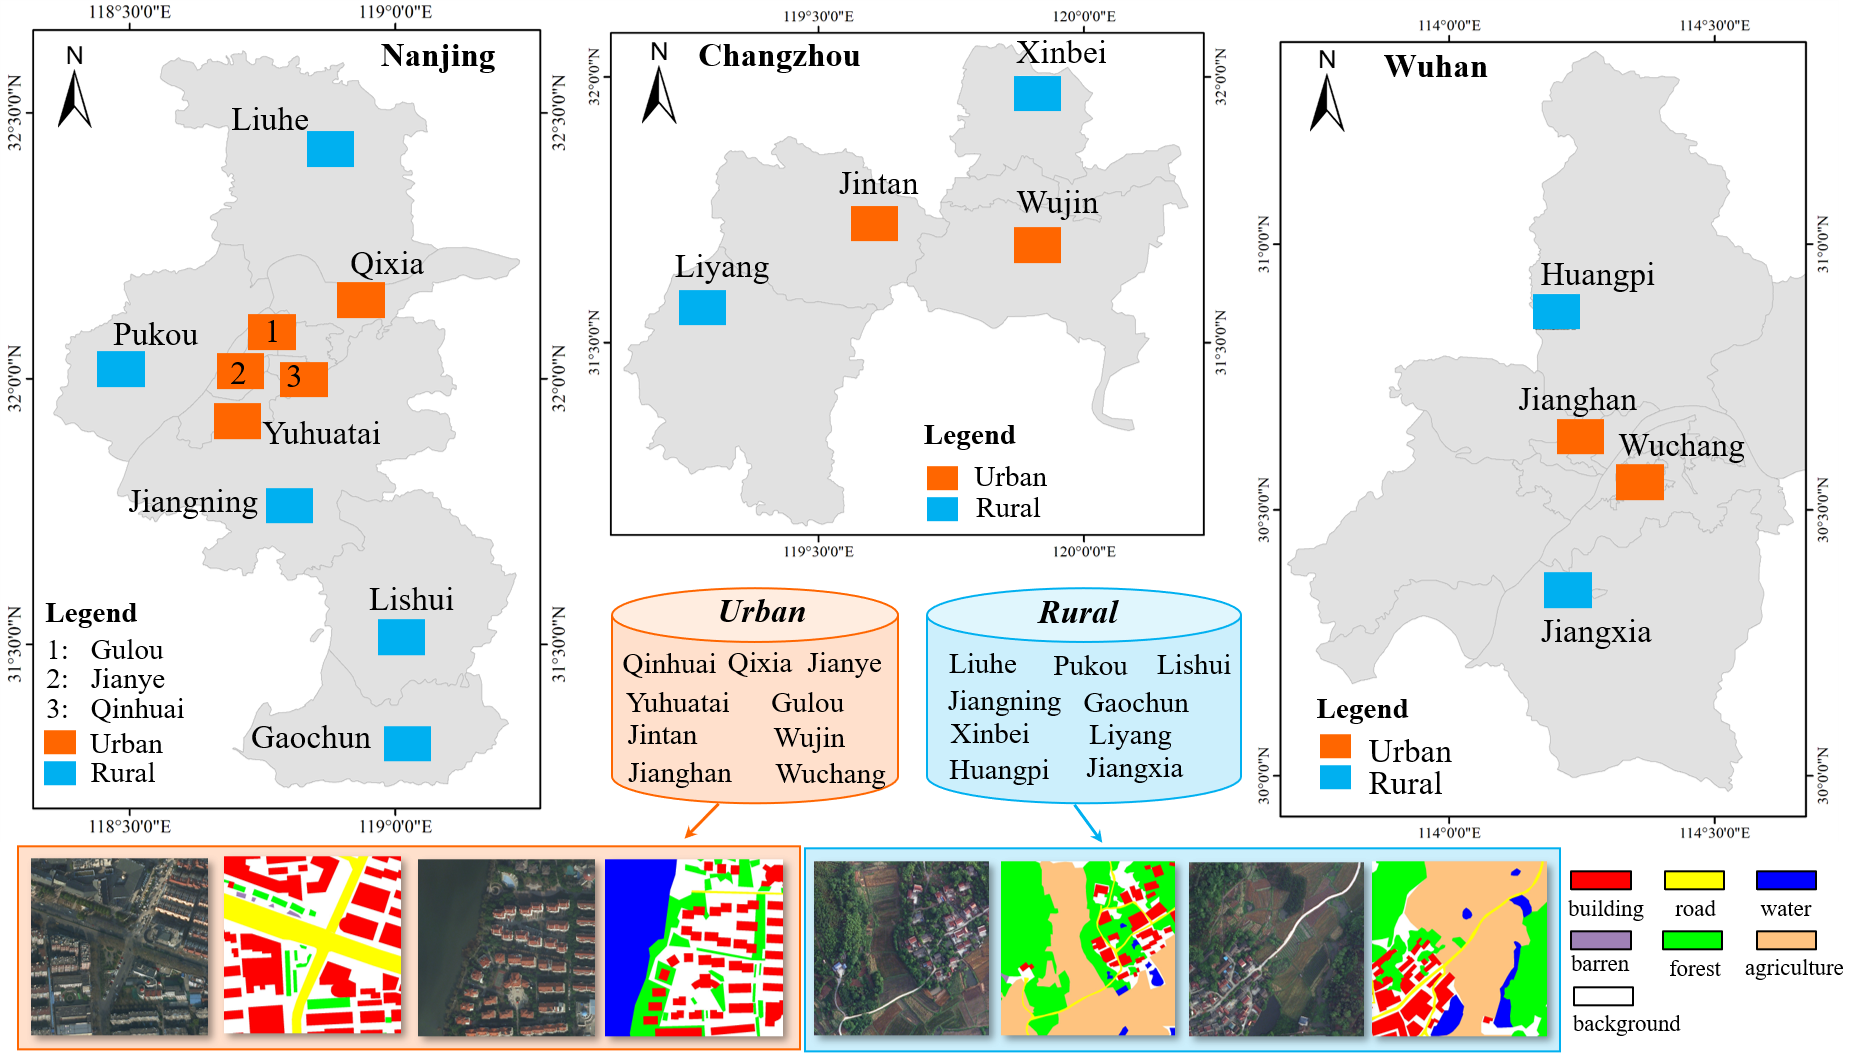
\includegraphics[width=\linewidth,trim=12bp 6bp 702bp 411bp,clip]{assets/course_imagery.png}
\small Urban example: image and annotation
\end{minipage}\hfill
\begin{minipage}{0.48\linewidth}\centering
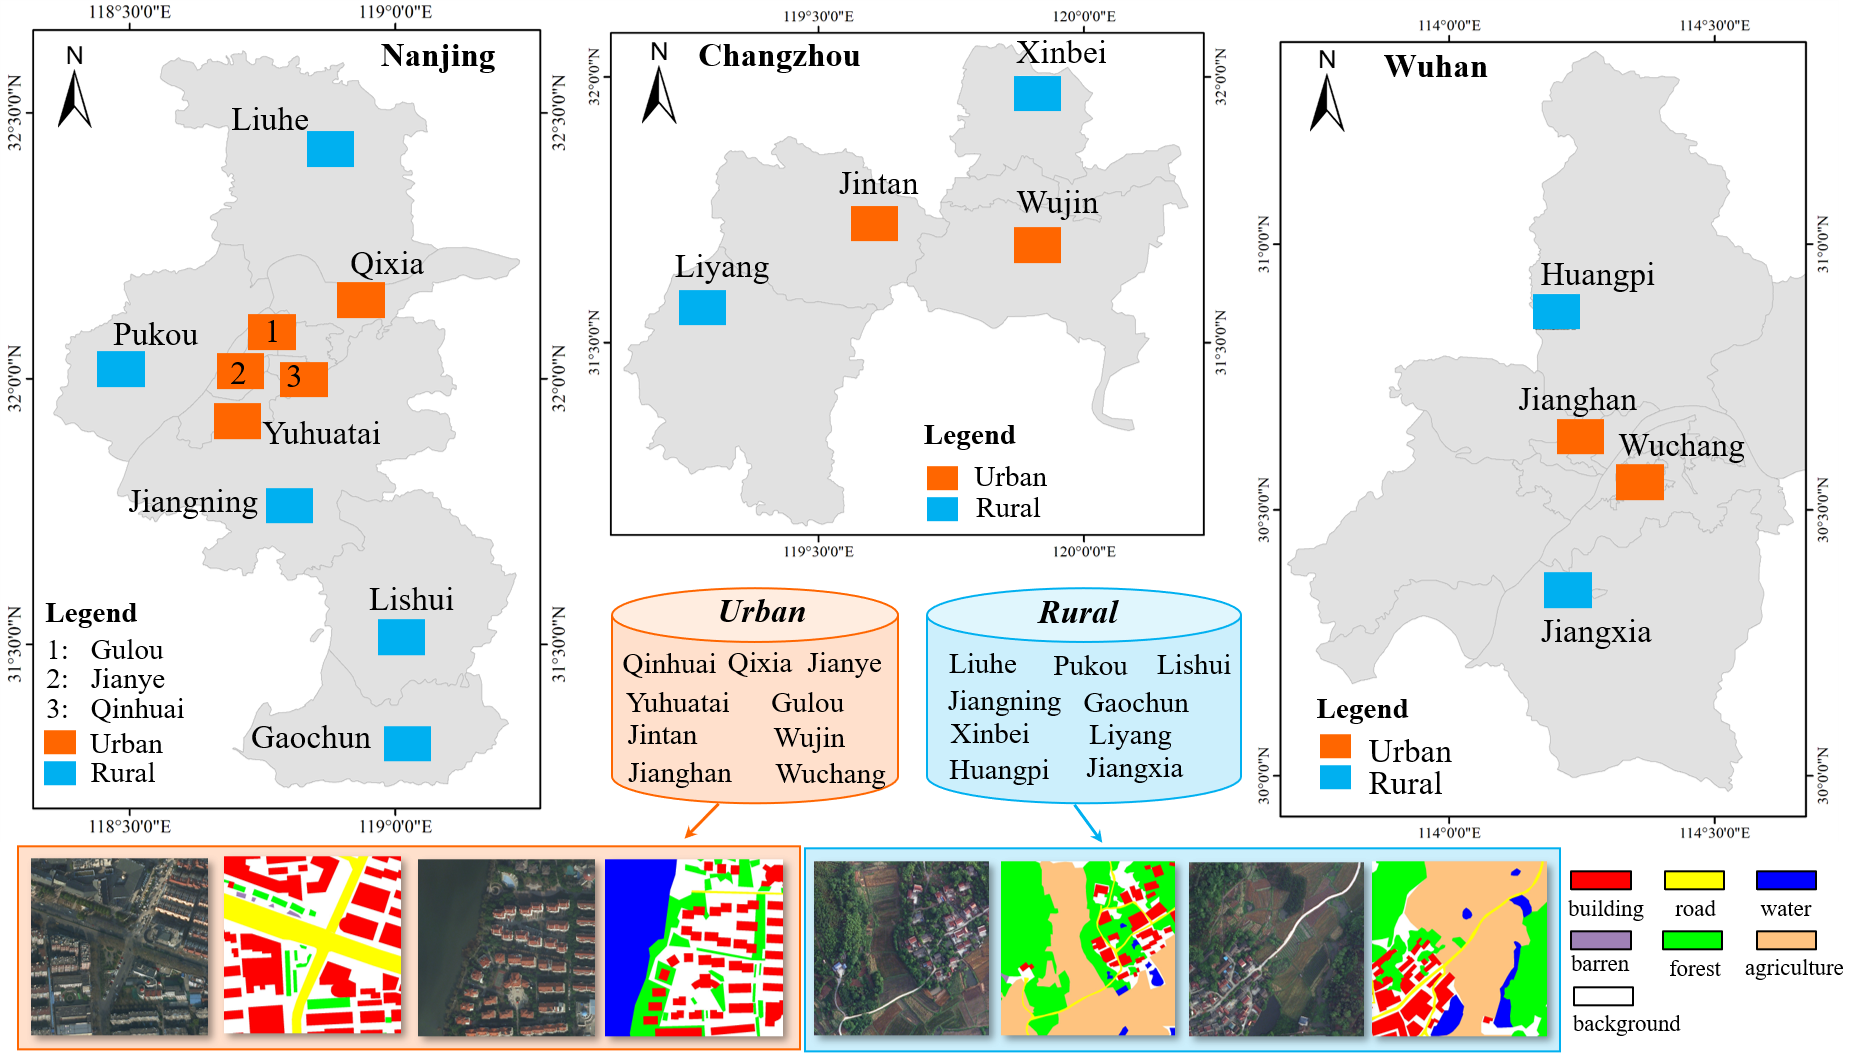
\includegraphics[width=\linewidth,trim=394bp 6bp 328bp 411bp,clip]{assets/course_imagery.png}
\small Rural example: image and annotation
\end{minipage}
\captionof{figure}{High-resolution satellite images and land-cover annotations, cropped in the page layout from Fig.~1 of Wang et al.~\cite{imagecredit}. Roads are yellow; this project predicts road versus non-road only. Figure credit: Wang et al.; source paper CC BY-NC-SA 4.0. Obtain project data from the course-provided package.}
\end{center}

\subsection{What you will build}
A \textbf{trainable recurrent transformer refiner} on top of a common, frozen initial segmenter. Submit one set of weights and code. Staff will run it for exactly $K=1,2,4$ refinement steps for ranking, and $K=0,6,8$ for diagnosis. The same checkpoint must support every $K$.

\begin{tcolorbox}[colback=lightgray,colframe=graytext]
\textbf{Release status.} This handout is an instructor-review draft. Before launch, staff must publish the course data package, frozen baseline and feature interface, split manifests, final resource caps, and confirmed deadlines. The companion code includes an \emph{untrained synthetic demo}, not a trained road segmenter. The proposed metrics and weights below are public; they must be frozen before competition starts.
\end{tcolorbox}
\smallnote{Reading route: concepts and design, Sections~2--4; evaluation, Sections~5--8; submission, Section~9; research expectations and grading, Sections~10--11; readings and checklist, Section~12.}

\page{A short introduction to transformers and loops}
\subsection{Start with three ideas}
\textbf{Features} are numerical descriptions learned from an image: edges, textures, or more abstract patterns. A \textbf{token} is a vector describing one location or patch. A \textbf{transformer block} lets tokens exchange information using attention, then updates each token with a small neural network. You do not need to have taken the transformer lectures to start this project.

For example, divide a feature map into $N$ locations, each represented by a vector of length $d$. Put them in a matrix $X\in\R^{N\times d}$. One attention head computes
\begin{equation}
 Q=XW_Q,\quad J=XW_J,\quad V=XW_V,\qquad
 \operatorname{Attention}(X)=\operatorname{softmax}_{\rm row}\!\left(\frac{QJ^\top}{\sqrt{d_h}}\right)V.
\end{equation}
Here $W_Q,W_J,W_V$ are learned matrices; $Q$ contains \emph{queries}, $J$ contains \emph{keys}, $V$ contains \emph{values}, and $d_h$ is the query/key vector length. Row-wise softmax converts each token's similarities into weights that sum to one. We use $J$ for keys to avoid confusing them with the loop count $K$. Multiple heads learn different information exchanges. Position information tells the model where tokens are located.

\subsection{Stacking is not the same as weight sharing}
\begin{center}
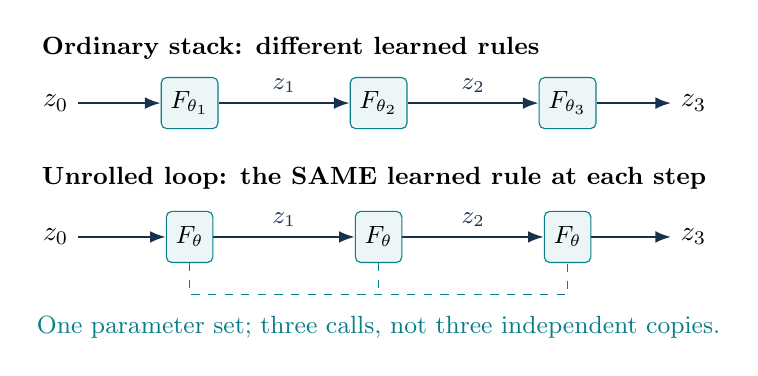
\begin{tikzpicture}[x=1cm,y=1cm]
\node[font=\small\bfseries,anchor=west] at (0,2.0) {Ordinary stack: different learned rules};
\node (a) at (0.3,1.3) {$z_0$};
\node[box] (b) at (2.0,1.3) {$F_{\theta_1}$};
\node[box] (c) at (4.4,1.3) {$F_{\theta_2}$};
\node[box] (d) at (6.8,1.3) {$F_{\theta_3}$};
\node (e) at (8.4,1.3) {$z_3$};
\draw[arr] (a)--(b);\draw[arr] (b)--node[above,font=\small]{$z_1$}(c);\draw[arr] (c)--node[above,font=\small]{$z_2$}(d);\draw[arr] (d)--(e);
\node[font=\small\bfseries,anchor=west] at (0,0.35) {Unrolled loop: the SAME learned rule at each step};
\node (a2) at (0.3,-0.4) {$z_0$};
\node[box] (b2) at (2.0,-0.4) {$F_{\theta}$};
\node[box] (c2) at (4.4,-0.4) {$F_{\theta}$};
\node[box] (d2) at (6.8,-0.4) {$F_{\theta}$};
\node (e2) at (8.4,-0.4) {$z_3$};
\draw[arr] (a2)--(b2);\draw[arr] (b2)--node[above,font=\small]{$z_1$}(c2);\draw[arr] (c2)--node[above,font=\small]{$z_2$}(d2);\draw[arr] (d2)--(e2);
\draw[teal,dashed] (b2.south)--++(0,-0.4)-|(d2.south);
\draw[teal,dashed] (c2.south)--++(0,-0.4);
\node[font=\small,color=teal] at (4.4,-1.55) {One parameter set; three calls, not three independent copies.};
\end{tikzpicture}
\captionof{figure}{Unrolling draws repeated calls as separate boxes for readability. In the loop, every box refers to the same module and the same parameter tensors.}
\end{center}

If one block has $p$ parameters, $K$ independent blocks have about $Kp$ parameters. Reusing one block keeps its parameter count at $p$, although its computation still grows approximately with $K$. The hidden state $z_t$ changes; the weights $\theta$ do not change during inference.

\begin{tcolorbox}
\textbf{What counts as reasoning here?} We use the narrower term \emph{iterative spatial inference}: a model uses context and its current state to revise a prediction. Shared weights do not prove reasoning, and more loops do not guarantee a better answer. Your experiments must test whether state and feedback actually matter.
\end{tcolorbox}
Universal Transformers motivate shared-depth attention~\cite{ut}. Tiny Recursive Models motivate repeatedly updating a latent state and a candidate answer~\cite{trm}. This project adapts these ideas; it is not a literal reproduction of either architecture.

\page{The model contract: one image, a changing state}
\subsection{Two different things change at each iteration}
For one image of height $H$ and width $W$ (omitting the batch dimension), $t$ counts completed refinement steps:
\begin{itemize}
\item \textbf{The current answer, $y_t\in\R^{H\times W}$:} one real-valued \emph{road logit} per pixel. A logit is an unrestricted score, not a probability: $p_t(u)=\sigma(y_t(u))=1/(1+e^{-y_t(u)})$ is the probability of road at pixel $u$. Thus $y_t$ is a dense prediction map, not a ground-truth label or a loss.
\item \textbf{The latent state, $z_t\in\R^{N_z\times d}$:} a bank of $N_z$ memory tokens, each a computed $d$-dimensional feature vector, not a road probability or model parameter. Tokens carry context between steps; a spatial state may keep one per coarse image patch. Their values change at inference; the model weights do not.
\end{itemize}
We reserve $g(u)\in\{0,1\}$ for ground truth and $L$ for loss. Ground truth never enters the inference loop. A frozen staff encoder and head produce $f=E(x)$ and $y_0=H_0(f)$ from RGB image $x$. Your initializer $I_\phi$ and shared update $R_\theta$ give
\begin{align}
 z_0 &= I_\phi(f,y_0),\\
 (z_{t+1},y_{t+1}) &= R_\theta(f,z_t,y_t),\quad t=0,\ldots,K-1,\label{eq:recurrence}\\
 p_K &= \sigma(y_K),\qquad P_K(u)=\ind[p_K(u)\geq0.5].
\end{align}
\textbf{What the transformer sees.} Inside $R_\theta$, adapters $T_x$ and $T_y$ embed image features and the current answer as token matrices: $X=T_x(f)\in\R^{N_x\times d}$ and $T_y(y_t)\in\R^{N_y\times d}$. $N_x,N_y$ count tokens; $d$ is their vector length. $y_t$ is \emph{tokenized before attention} and the new answer is decoded back to $H\times W$ logits. The tokenizers and output head are shared across steps.

\begin{center}
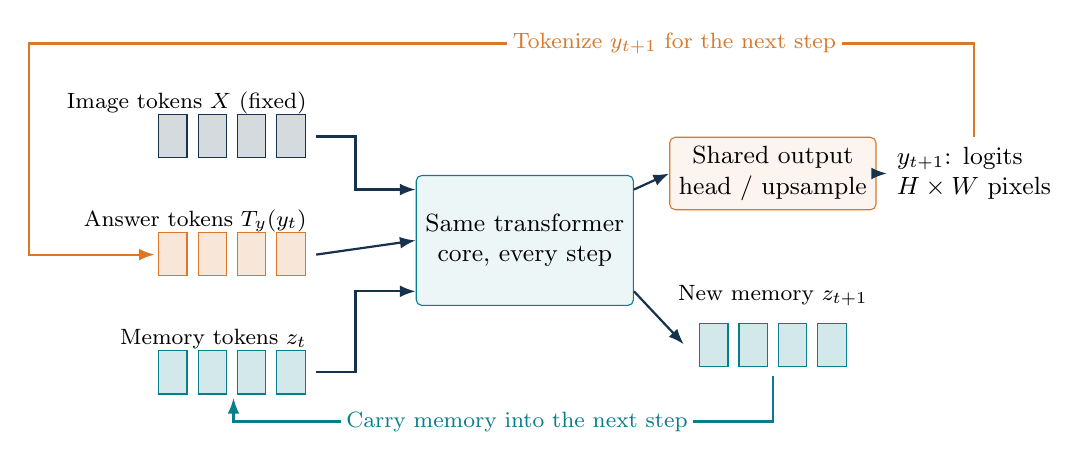
\begin{tikzpicture}[x=1cm,y=1cm]
\node[font=\footnotesize,anchor=east] at (2.55,2.05) {Image tokens $X$ (fixed)};
\node[font=\footnotesize,anchor=east] at (2.55,.55) {Answer tokens $T_y(y_t)$};
\node[font=\footnotesize,anchor=east] at (2.55,-.95) {Memory tokens $z_t$};
\foreach \yy/\col in {1.35/navy,-.15/orange,-1.65/teal}{
  \foreach \j in {0,...,3}{
    \filldraw[fill=\col!18,draw=\col] (0.55+\j*.5,\yy) rectangle ++(.36,.55);
  }
}
\node[box,minimum width=2.7cm,minimum height=1.65cm] (core) at (5.2,.3) {Same transformer\\core, every step};
\draw[arr] (2.55,1.62)--(3.05,1.62)|-(core.155);
\draw[arr] (2.55,.12)--(core.west);
\draw[arr] (2.55,-1.37)--(3.05,-1.37)|-(core.205);
\node[box,draw=orange,fill=orange!8,minimum width=2.0cm] (head) at (8.35,1.15) {Shared output\\head / upsample};
\node[font=\small,align=left,anchor=west] (answer) at (9.8,1.15) {$y_{t+1}$: logits\\$H\times W$ pixels};
\draw[arr] (core.25)--(head.west);\draw[arr] (head)--(answer);
\node[font=\footnotesize] at (8.35,-.4) {New memory $z_{t+1}$};
\foreach \j in {0,...,3}{
  \filldraw[fill=teal!18,draw=teal] (7.42+\j*.5,-1.3) rectangle ++(.36,.55);
}
\draw[arr] (core.-25)--(7.22,-1.02);
\draw[arr,draw=orange] (answer.north)|-(7.1,2.8)-|(-1.1,.12)--(.5,.12);
\node[font=\footnotesize,text=orange,fill=white,inner sep=2pt] at (7.1,2.8) {Tokenize $y_{t+1}$ for the next step};
\draw[arr,draw=teal] (8.35,-1.42)--(8.35,-2.0)--(1.5,-2.0)--(1.5,-1.7);
\node[font=\footnotesize,text=teal,fill=white,inner sep=2pt] at (5.1,-2.0) {Carry memory into the next step};
\end{tikzpicture}
\captionof{figure}{One update, inspired by TRM's input/answer/latent separation~\cite{trm}. Each small rectangle is a \emph{vector token}, not one pixel or a transformer layer. Token counts and fusion are design choices. This is a segmentation adaptation, not TRM's exact nested schedule.}
\end{center}

\subsection{Mandatory for the main competition}
\begin{itemize}
\item Reuse one core and all adapters; carry $z_t$ and feed back $y_t$. All student parameters count toward the budget. A fixed multi-layer core is allowed; independent per-step cores are not.
\item Run exactly $K$ updates with one checkpoint. At $K=0$, return the untouched staff prediction $\sigma(y_0)$. Freeze staff weights and normalization statistics.
\item No independent trainable U-Net/CNN segmentation bypass. Convolutions for tokenization, upsampling, and state-conditioned detail recovery are allowed.
\end{itemize}

\page{Design choices and a feasible starting route}
\small
\renewcommand{\arraystretch}{1.1}
\begin{tabularx}{\linewidth}{@{}>{\raggedright\arraybackslash}p{1.10in}YY@{}}
\toprule
Choice & Reasonable starting point & Research directions you may explore\\\midrule
State & Low-resolution feature grid & Two states; multiscale grids; learned memory tokens.\\
Attention & Local/window attention with image features & Coarse global attention; cross-attention; sparse links. Explain long-range communication.\\
Output update & Small correction to logits & Replacement logits; gated or uncertainty-aware updates. Residuals are optional.\\
Feedback & Previous logits and persistent state & Probability/uncertainty embeddings; learned fusion; feedback ablations.\\
Training & Short unroll, intermediate supervision & Random $K$; curriculum; truncated gradients; topology/boundary losses.\\
Stopping & Fixed exact $K$ for ranking & Adaptive halting as a separate experiment, never in ranking mode.\\
\bottomrule
\end{tabularx}
\normalsize

\subsection{A first implementation, before ambitious changes}
\begin{enumerate}
\item Verify raw labels and reproduce the frozen baseline on development data. Save both correct and failed road predictions.
\item Start with a $1/16$-resolution state, a small shared transformer, and a simple output head. Use crop-based training, not full-resolution global attention.
\item Overfit a tiny training subset to check gradients, ignore masks, and feedback. Then train a first $K=1,2,4$ model on the allowed training partition.
\item Change one meaningful design choice; evaluate the same checkpoint at all $K$. Track quality, time, memory, and failure cases.
\end{enumerate}

For a starting training objective, let $g(u)\in\{0,1\}$ be the ground-truth road label, $V$ the valid pixels, and $\mathcal T$ the supervised steps. The prediction is $p_t=\sigma(y_t)$:
\begin{align}
 L_{\rm BCE}(p,g)&=-\frac{1}{|V|}\sum_{u\in V}\left[g(u)\log p(u)+(1-g(u))\log(1-p(u))\right],\\
 L&=\sum_{t\in\mathcal T}w_t L_{\rm BCE}(p_t,g),\qquad w_t\geq0,\quad\sum_t w_t=1.
\end{align}
Use a numerically stable logits-based implementation; skip all-ignore crops. $w_t$ are training weights chosen by your team, not leaderboard weights. Soft-clDice is an optional differentiable training loss~\cite{cldice}; the hard evaluation skeleton in Section~5 is not differentiable.

\subsection{Memory matters on one GPU}
The target hardware is one NVIDIA L40S (48 GB device memory)~\cite{l40s}. A $512\times512$ crop at stride 16 has $32^2=1{,}024$ tokens. At full pixel resolution it has $262{,}144$ tokens. A dense attention matrix grows as $N^2$ per head; recurrence does not remove that cost. Training also stores activations across steps.

\smallnote{Proposed design targets, pending a staff pilot: at most 5M core parameters and 10M total student trainable parameters; aim for at most 32 GiB peak allocated training memory. Frozen staff weights are reported separately. Use mixed precision, small batches/gradient accumulation, window attention, or activation checkpointing as needed. Staff must announce final hard caps, GPU-hours, input/tile policy, and timeout before launch. No multi-GPU or outside-model advantage in the main track.}

\page{Evaluation I: overlap and centerlines}
\subsection{Inputs, labels, and counting conventions}
Evaluation uses original-resolution masks, without resizing the ground truth. In the supplied label files, 3 means road, 0 means no-data/ignore, and 1,2,4,5,6,7 are non-road. Use the course-provided files and this encoding; do not apply a library's label remapping twice.

For image $i$, let $L_i(u)$ be its raw label and define sets
\begin{equation}
 V_i=\{u:L_i(u)\ne0\},\quad G_i=\{u:L_i(u)=3\},\quad
 P_i=\{u:p_K^{(i)}(u)\geq0.5\}\cap V_i.
\end{equation}
$G_i$ is the ground-truth road set; $P_i$ is the predicted road set. The threshold is always 0.5. Ignore pixels never become positive or negative examples. Below, $D$ is a specified collection of images; $|M|$ is the number of pixels in a set $M$. Counts are summed across images \emph{before} division.

\subsection{1. Road intersection-over-union: how much road area is correct?}
Define $\mathrm{TP}=\sum_i|P_i\cap G_i|$, $\mathrm{FP}=\sum_i|P_i\setminus G_i|$, and $\mathrm{FN}=\sum_i|G_i\setminus P_i|$, where each sum is over $i\in D$. Then
\begin{equation}
 \operatorname{IoU}(D,K)=\frac{\mathrm{TP}}{\mathrm{TP}+\mathrm{FP}+\mathrm{FN}}
 =\frac{\sum_{i\in D}|P_i\cap G_i|}{\sum_{i\in D}|P_i\cup G_i|}.
\end{equation}
For example, 80 correctly predicted road pixels, 10 false road pixels, and 10 missed road pixels give $80/(80+10+10)=0.80$. Correctly classified background does not inflate this score.

\subsection{2. clDice: do the predicted and true centerlines stay inside roads?}
Skeletonization thins a binary region to a centerline. Let $S(M)$ be the 2D Zhang skeleton of $M$, as implemented by the pinned evaluator. Define
\begin{align}
 T_p&=\frac{\sum_{i\in D}|S(P_i)\cap G_i|}{\sum_{i\in D}|S(P_i)|},&
 T_s&=\frac{\sum_{i\in D}|S(G_i)\cap P_i|}{\sum_{i\in D}|S(G_i)|},\\
 \operatorname{clDice}(D,K)&=\frac{2T_pT_s}{T_p+T_s}.\label{eq:cldice}
\end{align}
$T_p$ asks whether the predicted centerline lies in true road; $T_s$ asks whether the true centerline is covered by predicted road. Their harmonic mean penalizes a weak value of either one~\cite{cldice}.

\begin{center}
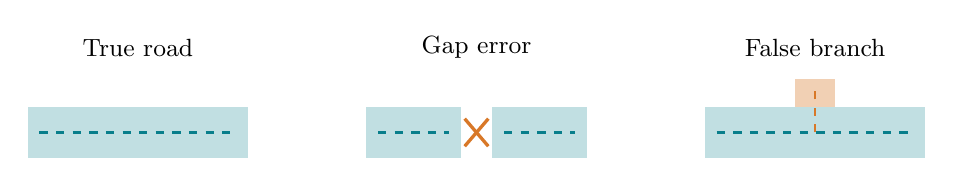
\begin{tikzpicture}[x=1cm,y=1cm]
\foreach \x/\lab in {0/True road,4.3/Gap error,8.6/False branch}{
\node[font=\small] at (\x+1.4,1.4) {\lab};}
\fill[teal!25] (0,0) rectangle (2.8,0.65);\draw[teal,thick,dashed] (0.15,.325)--(2.65,.325);
\fill[teal!25] (4.3,0) rectangle (5.5,.65);\fill[teal!25] (5.9,0) rectangle (7.1,.65);
\draw[teal,thick,dashed] (4.45,.325)--(5.35,.325);\draw[teal,thick,dashed] (6.05,.325)--(6.95,.325);
\draw[orange,very thick] (5.55,.15)--(5.85,.5);\draw[orange,very thick] (5.55,.5)--(5.85,.15);
\fill[teal!25] (8.6,0) rectangle (11.4,.65);\fill[orange!35] (9.75,.65) rectangle (10.25,1.0);
\draw[teal,thick,dashed] (8.75,.325)--(11.25,.325);\draw[orange,thick,dashed] (10,.325)--(10,.93);
\end{tikzpicture}
\captionof{figure}{Conceptual masks, not model results. Area overlap can hide a small but consequential gap. Centerline agreement adds a different view, but is not a direct measurement of global routability.}
\end{center}

\page{Evaluation II: boundaries and exact aggregation}
\subsection{3. Boundary IoU: are road edges in the right place?}
Let $E_3(M)$ erode a binary set $M$ using a $3\times3$ all-ones square for exactly three iterations, treating locations outside the image as zero. Erosion removes the outer layer of a foreground region at each iteration. Define the valid interior $C_i=E_3(V_i)$ and the inner boundary band
\begin{equation}
 B_i(M)=\bigl(M\setminus E_3(M)\bigr)\cap C_i.
\end{equation}
This gives a three-pixel band in the square-grid distance. $C_i$ excludes a three-pixel neighborhood of no-data and the image frame, so those artificial cuts are not scored as road edges. This is the course's fixed-width Boundary IoU variant, motivated by Cheng et al.~\cite{biou}; it is not a tunable tolerance.
\begin{equation}
 \operatorname{BIoU}(D,K)=
 \frac{\sum_{i\in D}|B_i(P_i)\cap B_i(G_i)|}
 {\sum_{i\in D}|B_i(P_i)\cup B_i(G_i)|}.
\end{equation}

\begin{center}
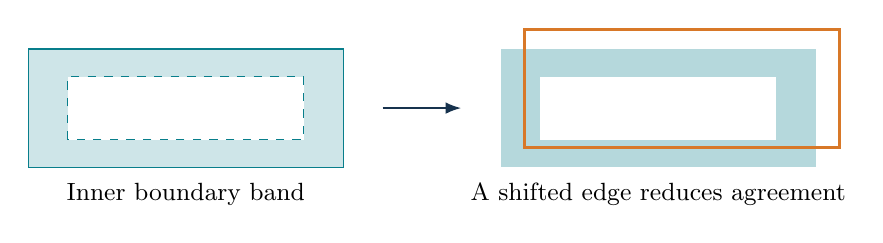
\begin{tikzpicture}[x=0.5cm,y=0.5cm]
\fill[teal!20] (0,0) rectangle (8,3);\fill[white] (1,.7) rectangle (7,2.3);
\draw[teal] (0,0) rectangle (8,3);\draw[teal,dashed] (1,.7) rectangle (7,2.3);
\node[font=\small] at (4,-.7) {Inner boundary band};
\draw[arr] (9,1.5)--(11,1.5);
\fill[teal!30] (12,0) rectangle (20,3);\fill[white] (13,.7) rectangle (19,2.3);
\draw[orange,very thick] (12.6,0.5) rectangle (20.6,3.5);
\node[font=\small,align=center] at (16,-.7) {A shifted edge reduces agreement};
\end{tikzpicture}
\captionof{figure}{The boundary metric measures overlap of narrow foreground edge bands, not full road interiors. The drawing is schematic; the code uses exactly three erosion iterations.}
\end{center}

\subsection{One quality number for any evaluation set and loop count}
All three metrics are fractions in $[0,1]$, with larger values better:
\begin{equation}
 \boxed{A(D,K)=0.50\operatorname{IoU}(D,K)+0.30\operatorname{clDice}(D,K)+0.20\operatorname{BIoU}(D,K).}\label{eq:quality}
\end{equation}
The weights balance road area, centerline coverage, and boundaries. This is a \emph{course-designed composite}, not a standard multiclass segmentation benchmark score. There are no additional hidden quality or robustness multipliers.

\subsection{Conventions that prevent implementation disagreements}
\begin{itemize}
\item Pool integer counts within $D$ first; do not average per-image scores. Empty tiles therefore do not each earn a separate perfect score. Overall scoring pools urban and rural together; also report both domains separately.
\item If an IoU union is empty, its value is 1. For $T_p$ or $T_s$, an empty denominator gives 1. If $T_p+T_s=0$, clDice is 0. Thus both road sets empty gives clDice 1; only one empty gives 0.
\item All-ignore images add zero counts. Reject an entire subset with no valid pixels. Skeletonize each valid-clipped mask separately; never connect neighboring tiles. No-data may cut centerlines, so interpret results near missing data cautiously.
\item Use hard Zhang skeletons, not a soft training approximation. A high clDice does not establish graph connectivity, road navigability, or human-like reasoning. Qualitative and controlled experiments remain necessary.
\end{itemize}

\page{The public leaderboard formula}
Let $\Oset$ contain unmodified evaluation images. Let $\Tset$ contain one controlled corrupted version of each of those images, with its original label. Section~8 defines the corruptions. The same four quality measurements determine every team's score:
\begin{equation}
\boxed{\begin{aligned}
\mathrm{Score}=100\big[&0.20A(\Oset,1)+0.20A(\Oset,2)\\
 &+0.40A(\Oset,4)+0.20A(\Tset,4)\big].
\end{aligned}}\label{eq:score}
\end{equation}
The range is 0--100. The first two terms reward useful early predictions; the third emphasizes the four-step result; the last tests robustness. \textbf{All weights, definitions, thresholds, and corruption ranges are public.} Only private evaluation instances and seeds are withheld.

\begin{center}
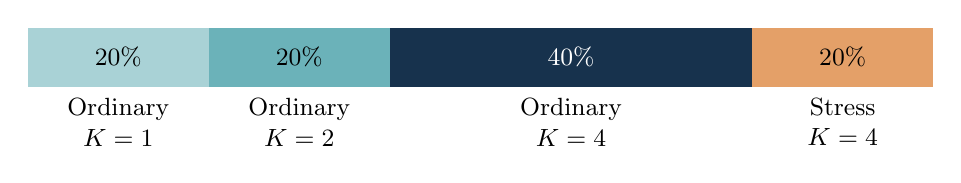
\begin{tikzpicture}[x=0.115cm,y=1cm]
\fill[teal!35] (0,0) rectangle (20,.75);
\fill[teal!60] (20,0) rectangle (40,.75);
\fill[navy] (40,0) rectangle (80,.75);
\fill[orange!70] (80,0) rectangle (100,.75);
\node[font=\small] at (10,.38) {20\%};\node[font=\small] at (30,.38) {20\%};
\node[font=\small,text=white] at (60,.38) {40\%};\node[font=\small] at (90,.38) {20\%};
\node[font=\small,align=center] at (10,-.45) {Ordinary\\$K=1$};
\node[font=\small,align=center] at (30,-.45) {Ordinary\\$K=2$};
\node[font=\small,align=center] at (60,-.45) {Ordinary\\$K=4$};
\node[font=\small,align=center] at (90,-.45) {Stress\\$K=4$};
\end{tikzpicture}
\captionof{figure}{How the final score allocates its weight. Each segment uses the same quality definition in Eq.~\eqref{eq:quality}.}
\end{center}

\subsection{A complete numerical example}
Suppose ordinary $K=4$ gives road IoU $0.72$, clDice $0.80$, and Boundary IoU $0.40$. Then
\[
 A(\Oset,4)=0.50(0.72)+0.30(0.80)+0.20(0.40)=0.68.
\]
If the other qualities are $A(\Oset,1)=0.60$, $A(\Oset,2)=0.64$, and $A(\Tset,4)=0.55$, then
\[
 \mathrm{Score}=100[0.20(0.60)+0.20(0.64)+0.40(0.68)+0.20(0.55)]=63.0.
\]
These are illustrative values, not measured baseline performance.

\subsection{What is reported but does not add another score multiplier?}
\begin{itemize}
\item $K=0$ staff baseline; $K=6,8$ extrapolation; every component at every $K$.
\item Refinement gain $\Delta_K=A(\Oset,K)-A(\Oset,0)$ and $A(\Oset,4)-A(\Oset,1)$. Gains may be negative. There is no reward for deliberately weakening an early prediction.
\item Urban/rural breakdown; ordinary/stress breakdown; parameter counts; latency; inference and training peak memory; training GPU-hours.
\end{itemize}
\textbf{Eligibility and quality are separate.} A strong U-Net without the required shared loop is not an eligible main entry. An eligible loop that fails to improve can still support a strong research report. No monotonic-improvement threshold is an eligibility test.

\page{Stress tests, data splits, and competition rules}
\subsection{A reproducible, disclosed stress suite}
Staff generate exactly one stress version per source tile. Within each domain, a seed-based permutation assigns shadow, occlusion, and blur as evenly as possible (counts differ by at most one). Locations do not use labels. The published \texttt{make\_stress.py} is the reference implementation:
\begin{center}\small
\begin{tabularx}{\linewidth}{@{}p{0.85in}X@{}}
\toprule
Family & Transformation at original image resolution\\\midrule
Shadow & One rectangle, requested area fraction uniformly in $[0.04,0.12]$ and aspect ratio in $[0.5,2]$. Multiply RGB inside by a factor uniformly in $[0.3,0.6]$.\\
Occlusion & One rectangle, area fraction uniformly in $[0.005,0.02]$, aspect ratio in $[0.5,2]$. Fill with the source image's per-channel median.\\
Blur & Gaussian blur of each RGB channel; standard deviation uniformly in $[1,2]$ pixels, reflected padding, kernel truncated at four standard deviations.\\
\bottomrule
\end{tabularx}\end{center}
For rectangle area fraction $a$ and width/height ratio $r$, choose height $h=\operatorname{round}(\sqrt{aHW/r})$ and width $w=\operatorname{round}(\sqrt{aHWr})$, each clamped to the image and at least one pixel. Sample its top-left corner uniformly over fitting integer locations. Clip RGB to $[0,1]$, multiply by 255, and round to save an 8-bit image. Seeds and exact rounding are fixed by the code and pinned dependencies.

The ground truth is unchanged; the frozen segmenter runs on the \emph{corrupted RGB input}. There is no oracle clean mask, clean feature cache, or paired clean image available during a stress run. Publish development examples and seeds. The stress set is a synthetic robustness test, not a substitute for natural domain shift. Some occluded content is genuinely unknowable; do not infer that every gap should be connected.

\subsection{The course-provided data}
Staff will provide a versioned collection of high-resolution RGB satellite-image tiles and pixel-aligned land-cover masks. Tiles are $1024\times1024$ pixels at approximately 0.3 m per pixel. Urban scenes contain dense buildings, intersections, and roads of different widths; rural scenes include fields, vegetation, water, and smaller roads. Shadows, visually similar surfaces, and different scene layouts make road extraction challenging.

The task is \textbf{binary road versus non-road segmentation}: other land-cover classes become non-road, and no-data is ignored. Download the course package from staff's announced location. Use its image IDs, checksums, and fixed split manifests. Keep every crop from a tile in that tile's assigned split. Do not obtain substitute images or annotations elsewhere.

\textbf{Allowed use.} Fit model weights on training data and choose settings/checkpoints on development data. Evaluation annotations are reserved for staff. Do not search for matching images or annotations elsewhere, reconstruct evaluation labels from external sources, or use evaluation labels for training or tuning. No extra labeled data, outside segmentation checkpoints, or test-time label access is allowed. Full data provenance and research-citation instructions will be supplied by staff for any publication; the course package does not imply staff created the underlying imagery.

\subsection{Public versus final ranking}
Proposed policy: reserve 30\% of course evaluation tiles for public feedback and 70\% for private ranking, stratified by domain. Compute Eq.~\eqref{eq:score} separately on each partition; do not blend their scores. Allow two submissions per team per day. Nominate \emph{one} checkpoint before private evaluation. Rank by full-precision private score, not displayed rounding. Staff rerun entries offline with resource limits.

\page{Submission interface: staff choose the loop count}
\subsection{One command, one checkpoint, exactly K updates}
The staff-owned runner handles image loading, repetition, output validation, and saving. Your team implements the model adapter in \texttt{submission/model.py} and submits safe tensor weights. Example official command, once the staff baseline is released:
\begin{lstlisting}
python predict.py --checkpoint submission/model.safetensors \
  --baseline staff/baseline.safetensors \
  --input evaluation/images --output predictions/k4 \
  --steps 4 --device cuda --save-trace
\end{lstlisting}
\texttt{--steps 0} returns the staff baseline, not your initializer's prediction. Ranking uses 1, 2, and 4. The runner also accepts 6 and 8, and never sends the requested total $K$ to your model. An adaptive-stopping experiment must use a separate interface; it cannot alter this command's exact-step meaning.

\begin{center}\small
\begin{tabularx}{\linewidth}{@{}>{\raggedright\arraybackslash}p{1.65in}Y@{}}
\toprule
Student interface & Responsibility\\\midrule
\texttt{build\_refiner(...)} & Construct all trainable modules once. Expose the shared transformer as \texttt{model.core}. Load the same state dictionary for all $K$.\\
\texttt{initialize(f, y0)} & Return the initial hidden state from features and initial logits. Do not call the recurrent core or run a separate full segmenter here.\\
\texttt{step(f, z, y)} & Take features, latent tokens $z_t$, and answer logits $y_t$; call the same core once; return $z_{t+1}$ and full-resolution $y_{t+1}$. No labels or total $K$.\\
\bottomrule
\end{tabularx}\end{center}
Features are staff-defined tensors; the demo uses five channels on a coarse grid. Logits must have shape $B\times1\times H\times W$. This starter runner processes one complete image at a time; any approved internal tiling must be deterministic, declared, and counted in compute. Staff must freeze the feature/tile contract before teams train.

\subsection{Files produced and checked}
For input \path{images/urban/001.png}, the ID is \path{urban/001}. Output includes a float32 $H\times W$ probability array at \path{probabilities/urban/001.npy}, a 0/255 PNG mask, and \texttt{run.json}. Probabilities must be finite and in $[0,1]$. With \texttt{--save-trace}, predictions $0,\ldots,K$ are saved. Evaluation thresholds probabilities at $p\geq0.5$, ignoring the submitted PNG.

The run manifest records image/checkpoint hashes, source hash, actual core calls, parameter counts, and diagnostic timing/memory. Missing, duplicate, mismatched, or invalid outputs fail validation. Hooks check core calls and parameter identity; they are not a proof against dishonest code. Staff also inspect source and run controlled interventions. No network or evaluation-label access is permitted.

\subsection{Try the included smoke test before real training}
\begin{lstlisting}
python smoke_test.py --output smoke_outputs
python -m unittest discover -s tests -v
\end{lstlisting}
\smallnote{The smoke test creates random weights and synthetic images, runs all four score components, and checks the combined result. It does not train a model. Official mode requires a staff baseline adapter. See the README for individual commands and manifests. Do not edit staff inference/evaluation code for official submissions.}

\page{Experiments: demonstrate understanding, not just accuracy}
\subsection{Required comparisons}
\begin{enumerate}
\item \textbf{Baseline and iteration curve.} Show the frozen baseline and your \emph{same} checkpoint at $K=1,2,4,6,8$. Plot each quality component against both $K$ and measured time. State which step counts were used in training.
\item \textbf{State/feedback interventions.} At inference, reset the hidden state before every update; separately replace mask feedback with the initial logits. Compare to the unmodified model. These interventions can create distribution shift, so treat them as diagnostics, not conclusive causal proof. Include a retrained no-feedback control when making a strong claim about learning to use feedback.
\item \textbf{A non-recurrent control.} Train a one-step model with approximately matched student parameter count. Also compare with an untied stack at approximately matched computation if feasible. A single control will generally not match both compute and parameters; report the mismatch rather than claiming it does.
\item \textbf{One hypothesis-driven design ablation.} Examples: local versus global context, residual versus replacement logits, intermediate losses, or a loop-count curriculum. Change one major factor and explain the expected outcome before running it.
\item \textbf{Failures and uncertainty.} Show unselected successes and failures, including false connections, disappearing roads, and later-step degradation. Report urban/rural and stress-family behavior. Where affordable, use three training seeds for the main claim; otherwise disclose the limitation and use paired image bootstrap intervals, noting spatial correlation.
\end{enumerate}

\subsection{How staff will check that it is genuinely a loop}
\begin{itemize}
\item Trace the computation at two different $K$: identical parameter objects/storage, repeated calls to one core, a changing carried state, and explicit mask feedback.
\item Check prefix consistency: steps 0--2 from a $K=4$ run should match a separate $K=2$ run with the same image/checkpoint/seed. The model must not choose a special branch for the final requested step.
\item Ask each team member to explain one update, distinguish state from parameters, follow tensor shapes, and predict what a state-reset or feedback removal should change.
\end{itemize}
Merely calling a transformer and discarding its output does not satisfy the project. Neither does allocating a new independent transformer per iteration. A module list is not automatically wrong: actual parameter reuse and dataflow, not the class name, decide compliance.

\subsection{What makes a strong research contribution?}
A focused, falsifiable claim supported by fair comparisons: for example, \emph{``Shared refinement helps recover thin road segments under shadows at the same inference budget, but over-connects parallel roads when unrolled too far.''} Explain the mechanism, alternative explanations, and limitations. A leaderboard improvement alone does not establish novelty or reasoning.

Promising teams can extend the study with another public road dataset, stronger compute-matched controls, multiple seeds, and an external holdout. Those are possible paper extensions, not a requirement to complete the course project. A submission-quality result is an aspiration; a well-executed negative result can earn an excellent course grade.

\page{Expectations, milestones, and grading}
\subsection{Teams and milestones}
Project A teams have \textbf{three students}. Share implementation, experiments, and interpretation; rotate roles so every member can explain the whole pipeline. Keep a contribution log and identify a primary owner and reviewer for each major experiment.
\begin{center}\small
\begin{tabularx}{\linewidth}{@{}p{1.25in}X@{}}
\toprule
When & Expected work\\\midrule
September 28 & Project Pitch Day (syllabus). Form a focused question and identify the first minimal experiment.\\
Before November 2 & Suggested ungraded checkpoint: label/CLI sanity tests, baseline reproduction, one shared update, and memory measurement. Staff should offer a short early transformer/recurrence tutorial.\\
November 2 & Proposal and midway update (syllabus): question, method diagram, initial results, resource plan, ablations, risks, and each member's contribution.\\
December 14--18 & Final presentation, report, code, and weights; exact date/time to be confirmed. No project assessment is due in the December 11--13 study period.\\
\bottomrule
\end{tabularx}\end{center}
\smallnote{The syllabus places RNNs on November 16 and Transformers I on November 18, after the midway deadline. Do not wait for those lectures to begin: use this primer, starter interface, and the proposed early tutorial.}

\subsection{Proposed project rubric (100 points, subject to instructor approval)}
\begin{center}\small
\begin{tabularx}{\linewidth}{@{}r p{1.5in}X@{}}
\toprule
Points & Component & What earns credit\\\midrule
10 & Question and proposal & Specific hypothesis, relevant reading, clear design and feasible plan.\\
15 & Midway work & Working loop, verified data pipeline, honest initial results, sensible response to failures.\\
30 & Final research report & Correct method, fair controls, meaningful ablations, uncertainty, error analysis, limitations, and supported conclusions.\\
15 & Reproducible implementation & Runnable code/weights, exact-$K$ behavior, environment, logs, compute accounting, and clean evaluation separation.\\
15 & Presentation and individual understanding & Clear explanation and live questions; every member understands recurrence, metrics, and their contributions.\\
15 & Leaderboard component & Valid final entry plus competitive ranking, defined below.\\
\bottomrule
\end{tabularx}\end{center}
For a valid final entry, assign $10+5(N-r)/(N-1)$ leaderboard points, where $N>1$ is the number of eligible teams and $r$ is rank (1 is best). Use mean ranks for exact ties. If $N=1$, assign 15. An invalid/missing entry receives 0 in this component, not automatically 0 for the entire project. Thus the best and worst eligible teams receive different ranking credit, while rigorous science remains most of the grade. The syllabus assigns the project 30\% of the course grade.

\subsection{Academic integrity and use of AI}
Follow the syllabus: AI may assist coding and research, but students own the creative decisions and must understand every submitted line. Write the report yourselves; AI use is limited to grammatical clarity. AI is not permitted for in-class presentations or quizzes. Cite external code, datasets, figures, and ideas; disclose tools and assistance. Do not share held-out labels, inspect evaluation annotations, or disguise pretrained/external models. Course late and academic-integrity policies apply.

\page{Reading guide and final checklist}
\subsection{Three papers to understand the central idea}
\begin{enumerate}
\item \textbf{Universal Transformers}~\cite{ut}: read the shared-depth update and its diagram. Ask: what changes between iterations, and what is reused?
\item \textbf{Less is More: Recursive Reasoning with Tiny Networks}~\cite{trm}: focus on latent-state and answer refinement. Its reasoning results do not establish that the approach works for road segmentation; that transfer is your research question.
\item \textbf{Recurrent Scene Parsing with Perspective Understanding in the Loop}~\cite{scene}: an earlier example of recurrent visual inference. Compare its feedback mechanism with your design. It is not itself a looped transformer.
\end{enumerate}
\subsection{Before the final submission}
\begin{itemize}
\item One nominated checkpoint, source code, pinned environment, training instructions, and a run manifest linking results to seeds/checkpoints.
\item A method diagram and parameter table; $K$-sweep and latency/memory measurements; all required controls; representative intermediate masks and failures.
\item Original report and slides in the course templates, with citations, limitations, contribution statement, and AI/code-use disclosures. Follow the course page limits when announced; do not replace evidence with architecture complexity.
\item Confirm that a fresh offline environment can run the exact command, with the same weights at all $K$, no downloads, and no labels available to inference.
\end{itemize}

\begingroup\small
\setlength{\parskip}{2pt}
\begin{thebibliography}{9}
\bibitem{imagecredit} J. Wang, Z. Zheng, A. Ma, X. Lu, and Y. Zhong. Source publication for Figure~1. NeurIPS Datasets and Benchmarks, 2021. \href{https://arxiv.org/abs/2110.08733}{Original publication and figure attribution}; \href{https://creativecommons.org/licenses/by-nc-sa/4.0/}{CC BY-NC-SA 4.0}. Display crops only; no claim of original imagery authorship by course staff.
\bibitem{ut} M. Dehghani, S. Gouws, O. Vinyals, J. Uszkoreit, and L. Kaiser. \emph{Universal Transformers}. ICLR, 2019. \url{https://arxiv.org/abs/1807.03819}.
\bibitem{trm} A. Jolicoeur-Martineau. \emph{Less is More: Recursive Reasoning with Tiny Networks}. arXiv, 2025. \url{https://arxiv.org/abs/2510.04871}.
\bibitem{scene} S. Kong and C. C. Fowlkes. \emph{Recurrent Scene Parsing with Perspective Understanding in the Loop}. CVPR, 2018. \url{https://arxiv.org/abs/1705.07238}.
\bibitem{cldice} S. Shit et al. \emph{clDice -- A Novel Topology-Preserving Loss Function for Tubular Structure Segmentation}. CVPR, 2021. \url{https://arxiv.org/abs/2003.07311}.
\bibitem{biou} B. Cheng, R. Girshick, P. Doll\'ar, A. C. Berg, and A. Kirillov. \emph{Boundary IoU: Improving Object-Centric Image Segmentation Evaluation}. CVPR, 2021. \url{https://arxiv.org/abs/2103.16562}.
\bibitem{l40s} NVIDIA. \emph{L40S GPU specifications}. \url{https://www.nvidia.com/en-us/data-center/l40s/}. Accessed August 29, 2026.
\end{thebibliography}
\endgroup
\end{document}
